\subsection{Exercise 1 - Lab 2}

\textbf{Mục tiêu \& Yêu cầu:}
\begin{itemize}
    \item Thiết kế mạch giao tiếp hai đèn LED 7 đoạn Anode chung với vi điều khiển STM32F103C6 sử dụng Transistor PNP (điều khiển qua các chân \texttt{EN0}, \texttt{EN1}) và các chân tín hiệu đoạn từ \texttt{PB0} đến \texttt{PB6}.
    \item Tận dụng lại hàm \texttt{display7SEG(int num)} từ Lab 1 để hiển thị số.
    \item Hiện thực mã nguồn trong hàm ngắt Timer Callback (\texttt{HAL\_TIM\_PeriodElapsedCallback}) để quét và hiển thị số \textbf{"1"} trên LED 7 đoạn thứ nhất và số \textbf{"2"} trên LED 7 đoạn thứ hai.
    \item Thời gian chuyển đổi (quét) giữa 2 LED là $0.5$ giây ($500\text{ms}$).
\end{itemize}

\vspace{0.3cm}

\textbf{Report 1: Sơ đồ nguyên lý (Schematic)}

\begin{center}
    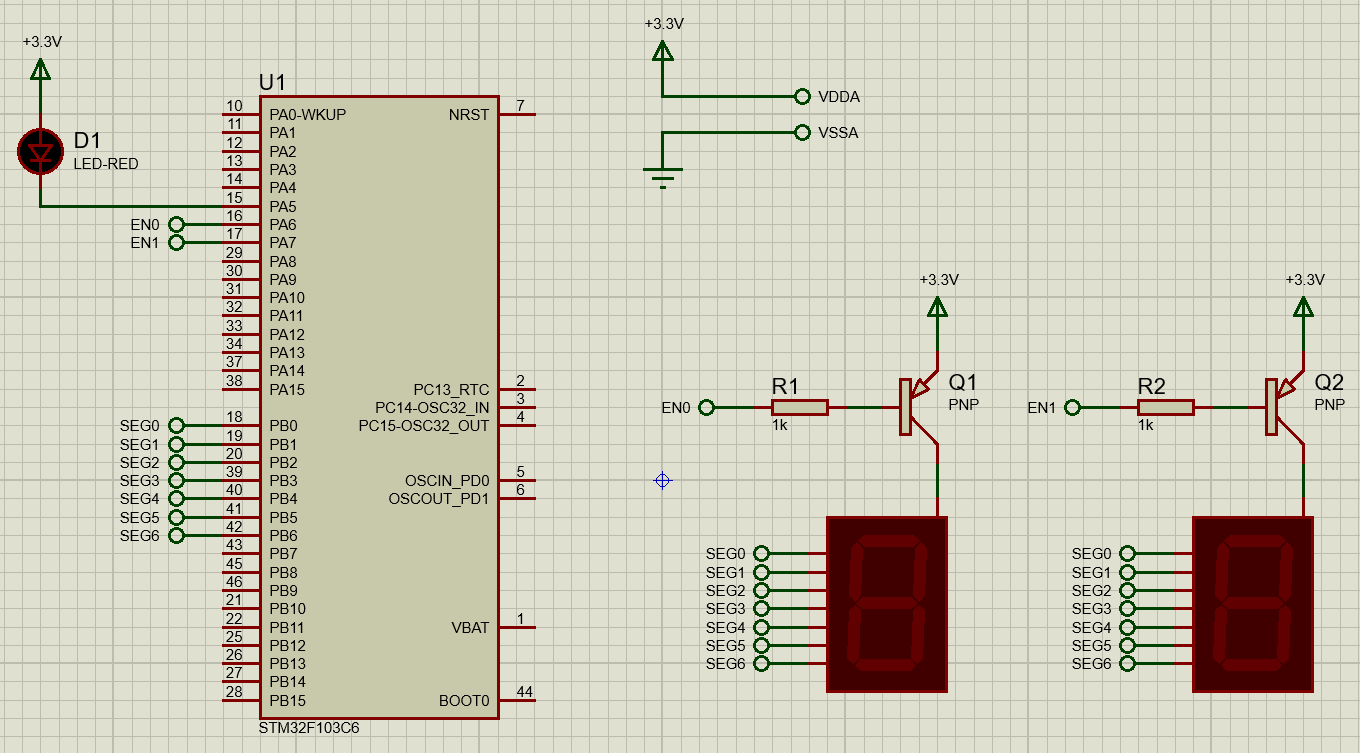
\includegraphics[width=9cm]{Picture/lab2_ex1.png}\\[0.2cm]
    {\small \textit{Hình 2.1: Sơ đồ mạch mô phỏng Proteus giao tiếp 2 LED 7 đoạn (Link Proteus: \href{https://github.com/lanton0403/VXL_VDK_Lab/raw/refs/heads/main/Lab_2/Exercise_1/Proteus/Lab2_1.pdsprj}{Download})}}
\end{center}

\vspace{0.3cm}

\textbf{Report 2: Mã nguồn trong hàm ngắt Timer Callback}

Đoạn mã xử lý luân phiên quét 2 LED 7 đoạn mỗi $500\text{ms}$ triển khai trong hàm \texttt{HAL\_TIM\_PeriodElapsedCallback}:

\begin{lstlisting}[language=C, caption={Hàm ngắt Timer điều khiển quét 2 LED 7 đoạn hiển thị số 1 và 2}, label={lst:lab2_ex1_code}]
/* USER CODE BEGIN 4 */
int led = 0;
int counter = 50;

void HAL_TIM_PeriodElapsedCallback(TIM_HandleTypeDef *htim)
{
    if (htim->Instance == TIM2)
    {
        counter--;
        if (counter <= 0)
        {
            counter = 50;

            if (led == 0)
            {
                HAL_GPIO_WritePin(GPIOA, EN1_Pin, GPIO_PIN_SET);
                display7SEG(1);
                HAL_GPIO_WritePin(GPIOA, EN0_Pin, GPIO_PIN_RESET);

                led = 1;
            }
            else
            {
                HAL_GPIO_WritePin(GPIOA, EN0_Pin, GPIO_PIN_SET);
                display7SEG(2);
                HAL_GPIO_WritePin(GPIOA, EN1_Pin, GPIO_PIN_RESET);

                led = 0;
            }
        }
    }
}
/* USER CODE END 4 */

\end{lstlisting}

\vspace{0.3cm}

\textbf{Short question: Tần số của quá trình quét LED là bao nhiêu?}
\begin{itemize}
    \item \textbf{Trả lời:} 
    Chu kỳ quét cho từng LED là $T_S = 0.5\text{s}$ ($500\text{ms}$). Do hệ thống quét luân phiên $2$ LED 7 đoạn, tổng chu kỳ quét hoàn chỉnh toàn bộ màn hình là:
    $$T_{scan} = 2 \times T_S = 2 \times 0.5\text{s} = 1.0\text{s}$$
    Tần số của quá trình quét (Scanning Frequency) là:
    $$f_{scan} = \frac{1}{T_{scan}} = \frac{1}{1.0\text{s}} = 1\text{Hz}$$
\end{itemize}